\section*{Expresividad}
La \textbf{expresividad} de un lenguaje nos determina la amplitud de las ideas que pueden ser representadas y comunicadas en él. En los lenguajes de consulta equivale al conjunto de consultas que se pueden expresar usándolos.

\subsection*{Expresividad de CRT}
CRT es una especialización particular de la \textbf{LPO} (Lógica de Primer Orden) adaptada a bases de datos, donde a cada instancia se le asocia un valor de verdad según si cumple con el predicado de la expresión de la consulta. En su semántica sólo buscamos saber la validez de la fórmula en la DB. \\
Dada una expresión, su \textbf{dominio} es el conjunto de valores que aparecen en ella como constantes o existen en cualquiera de las tuplas de las relaciones a las que hace referencia. Decimos que es \textbf{segura} si garantiza producir una cantidad finita de tuplas como resultado. Ejemplo de expresión insegura:
\begin{SQL}
    \{t | $\lnot$(t $\in$ EMPLEADO)\}
\end{SQL}
Alternativamente, en una expresión segura todos los valores en el resultado son parte del dominio de la expresión.

\textbf{Proposición:} CRT restringido a expresiones seguras tiene el mismo poder de expresividad que AR.

\textbf{DRC (Cálculo Relacional de Dominio):} A diferencia de CRT usa atributos en lugar de variables. Tiene el mismo poder expresivo.

\subsection*{Límites de la expresividad}
Hay consultas sobre las DB que no son expresables a través de AR ni CRT (incluso LPO). Podemos demostrar si una lo es o no a través de ciertas herramientas matemáticas. Para LPO tenemos el \textbf{teorema de Ehrenfeucht-Fraisse}.

\begin{figure}[H]
    \centering
    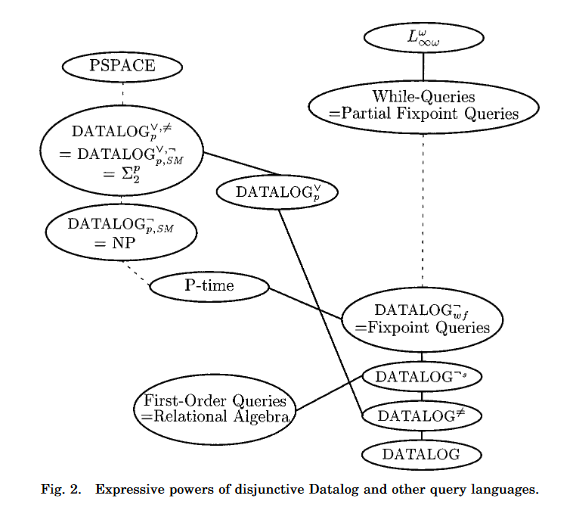
\includegraphics[scale=0.7]{fig/poder-expresivo.png}
\end{figure}

\subsubsection*{Teorema de Ehrenfeucht-Fraisse}
Es una demostración basada en Teoría de Juegos que se usa para determinar si dos estructuras son \textbf{elementalmente equivalentes} (isomorfas). Cuenta con dos jugadores: Spoiler y Duplicator, y dos estructuras (grafos): A y B. Se juega por rondas y en cada una Spoiler elige un nodo de una estructura y en respuesta Duplicator debe elegir uno de la otra. \\
Spoiler busca demostrar que las estructuras son \textbf{distinguibles}, mientras que Duplicator busca lo contrario. Dadas n rondas los grafos son \textbf{indistinguibles} si a partir de los nodos elegidos de cada estructura se tiene un isomorfismo parcial (se mantiene la igualdad y adyacencia). Si para n rondas Duplicator tiene estrategia ganadora decimos que:
\begin{center}
    A $\sim$n B
\end{center}
Ahora, las estrategias se pueden expresar a través de fórmulas de LPO donde la cantidad de rondas se corresponde con la cantidad de cuantificadores. Por ende, si A $\sim$n B luego A y B cumplen las mismas sentencias con n cuantificadores. Generalizado a la LPO:

\textbf{Teorema:} \textit{Una propiedad P no es expresable en la LPO si para todo n natural se pueden hallar dos grafos A y B tales que P sea falsa en A, verdadera en B y A $\sim$n B.}

Hay predicados \quotes{extra-lógicos} en SQL que permiten expandir su poder expresivo: recursión, funciones de agregación y agregamiento, operaciones aritméticas sobre atributos numéricos, store procedures.
